%%%%%%%%%%%%%%%%%%%%%%% file template.tex %%%%%%%%%%%%%%%%%%%%%%%%%
%
% This is a general template file for the LaTeX package SVJour3
% for Springer journals.          Springer Heidelberg 2010/09/16
%
% Copy it to a new file with a new name and use it as the basis
% for your article. Delete % signs as needed.
%
% This template includes a few options for different layouts and
% content for various journals. Please consult a previous issue of
% your journal as needed.
%
%%%%%%%%%%%%%%%%%%%%%%%%%%%%%%%%%%%%%%%%%%%%%%%%%%%%%%%%%%%%%%%%%%%
%
% First comes an example EPS file -- just ignore it and
% proceed on the \documentclass line
% your LaTeX will extract the file if required
\begin{filecontents*}{example.eps}
%!PS-Adobe-3.0 EPSF-3.0
%%BoundingBox: 19 19 221 221
%%CreationDate: Mon Sep 29 1997
%%Creator: programmed by hand (JK)
%%EndComments
gsave
newpath
  20 20 moveto
  20 220 lineto
  220 220 lineto
  220 20 lineto
closepath
2 setlinewidth
gsave
  .4 setgray fill
grestore
stroke
grestore
\end{filecontents*}
%
\RequirePackage{fix-cm}
%
%\documentclass{svjour3}                     % onecolumn (standard format)
%\documentclass[smallcondensed]{svjour3}     % onecolumn (ditto)
%\documentclass[smallextended]{svjour3}       % onecolumn (second format)
\documentclass[twocolumn]{svjour3}          % twocolumn
%
\smartqed  % flush right qed marks, e.g. at end of proof
%
\usepackage{graphicx}
%
% \usepackage{mathptmx}      % use Times fonts if available on your TeX system
%
% insert here the call for the packages your document requires
%\usepackage{latexsym}
% etc.
\usepackage{url}

%
% please place your own definitions here and don't use \def but
% \newcommand{}{}
%
% Insert the name of "your journal" with
\journalname{Environmental Earth Sciences}
%
\begin{document}

\title{TESSIN VISLab - Laboratory for Scientific Visualization%\thanks{Grants or other notes
%about the article that should go on the front page should be
%placed here. General acknowledgments should be placed at the end of the article.}
}
%\subtitle{Do you have a subtitle?\\ If so, write it here}

%\titlerunning{Short form of title}        % if too long for running head

\author{Lars Bilke         \and
        Carolin Helbig     \and
        Thomas Kalbacher   \and
        Olaf Kolditz       \and
        Dmitry Naumov      \and
        Karsten Rink       \and
        Agnes Sachse       \and
        Benny Selle        \and
        Alexander Singer   \and
        Feng Sun           \and
        Nico Trauth        \and
        Marc Walther       \and
        Norihiro Watanabe  \and
        Bj\"orn Zehner     \and
        Jennifer Ziesch
}

%\authorrunning{Short form of author list} % if too long for running head

\institute{L. Bilke \and C. Helbig \and T. Kalbacher \and O. Kolditz \and
           Dmitry Naumov \and Karsten Rink \and Agnes Sachse \and Alexander Singer
           \and Nico Trauth \and Marc Walther \and Norihiro Watanabe \at
              Department of Environmental Informatics, \\
              Helmholtz Centre for Environmental Research, \\
              Leipzig, Germany, \\
              \email{lars.bilke@ufz.de}           %  \\
%             \emph{Present address:} of F. Author  %  if needed
           \and
           O. Kolditz \at
              Applied Environmental System Analysis, \\
              Technische University at Dresden, \\
              Dresden, Germany
           \and
           B. Selle \at
           \and
           F. Sun \at
              Beijing Hydrological Center, \\
              Beijing, China
           \and
           B. Zehner \at
              Bundesanstalt für Geowissenschaften und Rohstoffe, \\
              Hannover, Germany
           \and
           J. Ziesch \at
              Leibniz Institute for Applied Geophysics, \\
              Hannover, Germany
}

\date{Received: date / Accepted: date}
% The correct dates will be entered by the editor


\maketitle

\begin{abstract}
Scientific visualization plays an important role in understanding data
and simulation results. A high-resolution stereoscopic virtual reality
(VR) environment is used to help scientists to explore large and complex
data sets, to be able to collaborate in workgroups containing people of
different backgrounds and to present results of a research project to
stakeholders or the public. The requirements for the computing equipment
driving the VR environment are forcing us to use specialized
software applications which can run in a parallel fashion (clustered)
and thus challenging us to find a good data workflow from source data
sets onto the display system. Therefore we develop software applications
like the OpenGeoSys Data Explorer and custom data conversion tools for
established visualization packages such as ParaView and VTK. A
presentation of a broad range of visualization case studies prove our
workflows. An outlook on how visualization techniques can be deeply
integrated into the simulation process is given and future technical
improvements such as a simplified hardware setup and useful interaction
techniques are outlined.
\keywords{Virtual Reality  \and  Visualization  \and  Computer Graphics}
% \PACS{PACS code1 \and PACS code2 \and more}
% \subclass{MSC code1 \and MSC code2 \and more}
\end{abstract}

%%%%%%%%%%
%% CONTENT
%%%%%%%%%%

\section{Introduction}
\label{introduction}

The TESSIN VISLab is a high-resolution immersive virtual reality
environment and was established in 2008 to face the need of analyzing
and working on increasingly complex data sets used to and generated by
simulations of natural phenomena in environmental sciences. Typical use
cases for this environment are:

\begin{itemize}
\itemsep1pt\parskip0pt\parsep0pt
\item
  collaborative discussions in a small group of scientists
\item
  exploring complex data sets
\item
  quality checking of data sets
\item
  showing concurrent visualizations of diverse integrated data sets
\item
  presenting research results to stakeholders
\item
  presenting to the general public such as on open day events
\end{itemize}

\subsection{Existing Vislabs}
\label{existing-vislabs}

\begin{itemize}
\itemsep1pt\parskip0pt\parsep0pt
\item
  Potsdam
\item
  Zuse Berlin
\item
  Magdeburg
\item
  Aachen
\end{itemize}

\section{TESSIN VISLab}
\label{tessin-vislab}

\subsection{Technical Overview}
\label{technical-overview}

The hardware setup of the TESSIN VISLab (shown above) uses a back
projection-based stereoscopic visualization environment with an
approximately 6x3 meter large main screen and extending projections
on the floor and two side wings. In order to achieve a high resolution
of approximately 6400x1800 pixels, 13 projectors are used.
Images are generated alternating for the left and the right eye
and users wear special glasses which separate these images, resulting in
a stereoscopic view. For the stereo separation we can switch
between two technologies -- active stereo using shutter glasses and
passive stereo using Infitec\cite{infitec} technology. We use an optical tracking
system, compensating for movement of the observer. Images are computed
such that correct perspective is maintained. A pointer device (Flystick) allows for
interaction with the virtual environment. The rendering is performed
using a cluster with 13 workstations (one for each projector) equipped
with high-end NVidia graphics boards (GPUs) and situated in a server
room aside. The master/server process of the actual application is
started on a KVM-terminal (connected to machines in the server room) in
front of the display. In addition to the virtual reality capabilities,
the VISLab can be employed for enhanced multimedia presentations such as
the simultaneous display of images, videos and documents.

As of the clustered setup we can only use software which can run in
parallel and synchronized. For showing visualizations we use the
software packages VRED, ParaView or Unity in conjunction with MiddleVR.

\subsection{Mobile VR equipment}
\label{mobile-vr-equipment}

For off-site presentations such as on conferences, workshops or project
partner visits we can utilize mobile equipment to demonstrate the same
visualizations as in the VISLab. The equipment consists of notebooks
with dedicated GPUs and 3D-enabled projectors or head-mounted displays
(HMDs) such as the Oculus Rift.

\begin{figure}
  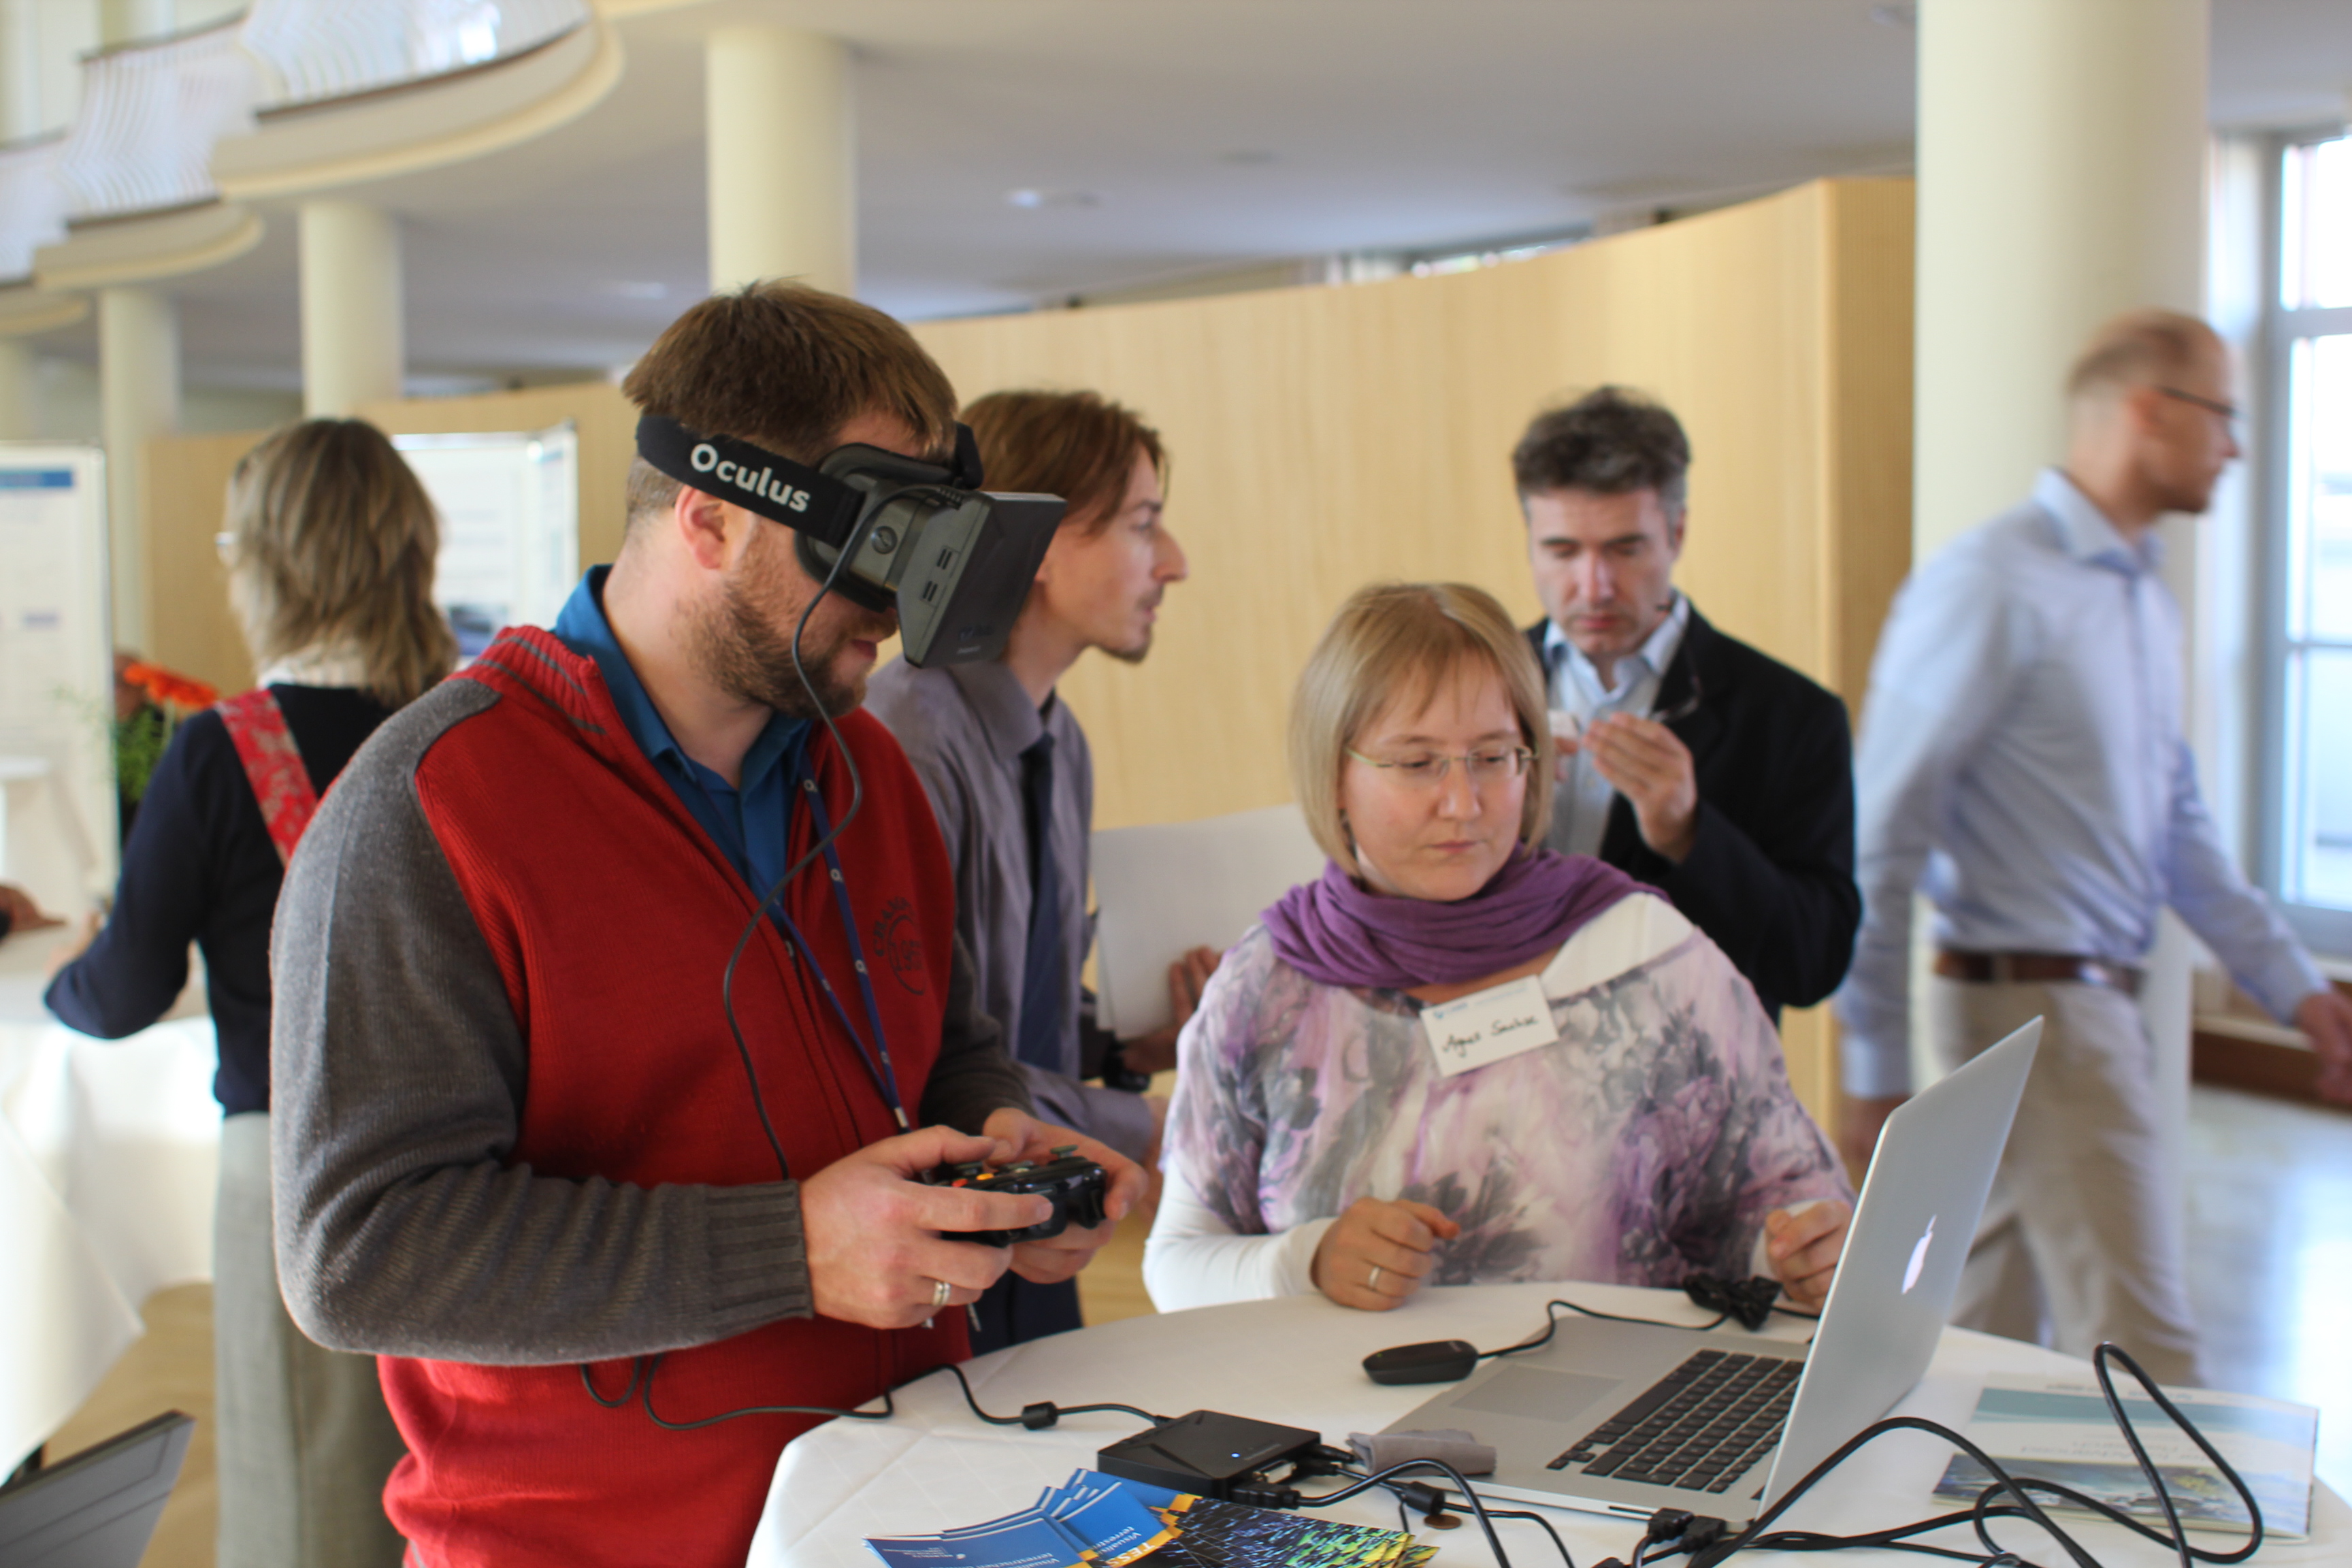
\includegraphics[width=\linewidth]{images/rift.jpg}
\caption{Mobile presentation at a scientific conference}
\label{fig:rift}
\end{figure}

\subsection{Software}
\label{software}

The following software is running on our display:

\paragraph{VRED}
is a commercial software by Autodesk (former PI-VR) specialized in
photorealistic real-time product rendering running on Windows. It is
build on top of OpenSG, an open-source scenegraph library which offers
clustered rendering \cite{opensg}. VRED can arrange imported 3D
objects in a virtual scene, allows for tweaking of material and lighting
parameters but is neither a modeling software nor are there many
interaction possibilities. It has a plugin interface but no
documentation on how to address it. An advantage is that VREDs editor
can be directly connected to the VISLabs display so that changes in the
scene are visible immediately. VRED is installed on the VISLab since
2008.

\paragraph{ParaView}\cite{paraview}
is an open-source data analysis and visualization software build on top of the
Visualization Toolkit\cite{vtk} (VTK). Both technologies also play an important in
our visualization workflows (see \ref{workflows}). ParaView allows to quickly
create visualizations and implements a large number of well established
visualization algorithms and techniques. It can run on distributed memory
architectures to analyze large data sets and to drive VR displays. Using
ParaView we can modify visualization parameters directly in the VR environment
but it lacks more sophisticated interaction and presentation feautures.

\paragraph{Unity}
is a complete game engine by Unity Technologies. It comes in a free and
a commercial editor variant. Unity has several rendering backends
(e.g.~OpenGL, OpenGL ES, DirectX) so it can be run on all major
platforms as well as on the Web (with an additional browser plugin).
From the first Unity does not provide any interaction functionality but
it has a comprehensive scripting documentation and a vivid plugin
community so that it is very easy to get started. Application testing
can be done directly in the Unity editor by tweaking the application at
runtime. However Unity created applications cannot run in a clustered
environment. Therefore MiddleVR is used.

\paragraph{MiddleVR}
is a generic virtual reality middleware from ``i'm in VR'' designed to
work with different 3D applications. It features a graphical
configuration tool to setup VR systems in a software independent way. It
handles interaction devices, stereoscopic rendering and clustering. Then
this configuration is used in a Unity plugin to enable all these
features in a Unity application. The MiddleVR enabled Unity application
is VR system agnostic, once compiled it can be run on any VR system
supported by MiddleVR. A disadvantage of this approach is that the final
application is not run inside the Unity editor but standalone so that it
cannot be altered interactively. The fact that a recompilation of the
application takes just a few seconds weakens that drawback. MiddleVR is
installed on the VISLab since 2014.

For the future we will focus on the use of Unity for highly interactive
presentations of visualizations as a platform to explain complex circumstances
and to help discussing methologies. For rapid prototyping and exploration of
visualizations ParaView is very useful.

As alternatives to software with native cluster rendering capabilities there are
middlewares which intercepts graphic commands from a desktop application and
redistributes them to a render cluster such as
Techviz\footnote{Techviz: \url{http://www.techviz.net/products/techviz-xl-driver/}} or
Conduit\footnote{Conduit: \url{http://www.mechdyne.com/conduit.aspx}}. Such
middleware software allow to run a regular 3D desktop application in a VR
environment with stereoscopy and tracking enabled. A data conversion is not
necessary but interaction and presentation techniques are limited by the desktop
application and performance is lost during graphic commands interception and
distribution to the cluster.

\subsection{Workflows}
\label{workflows}

TODO Datenquellen

TODO Simulation software OpenGeoSys \cite{kolditz:ogs}

As the foundation for our visualizations we use VTK which is
integrated into our in-house developed OGS Data Explorer framework
\cite{rink:eesenvirvis} as well as ParaView.

We provide conversion tools and ParaView plugins to adapt VTK
visualization data to formats needed for the display in the VISLab such
as OpenSG for VRED \cite{bilke:vtkosgconverter} and Autodesk FBX for
Unity \cite{bilke:vtkfbxconverter}. Conversion can be done manually in the
OGS Data Explorer as well as in an automated way with ParaView's Python
scripting interface which can be useful especially when converting time
series data. During conversion meta data is appended to the data sets to
include information not necessarily supported in FBX such as which
shader setup to use or time stepping information. The meta data is
evaluated when loading the data into Unity and can be queried, e.g.~for
displaying the time stepping information as a text overlay. Multiple
data sets can be arranged both in a spatial but also in a temporal
context. Viewing positions and camera animations can be predefined.
Additionally we implemented functionality in Unity to fade in/out data
sets, to select subsets, \ldots{} TODO \ldots{}

\section{Overview of VISLab Applications}
\label{overview-of-vislab-applications}

\subsection{Hydrology and Climate}
\label{hydrology-and-climate}

The challenge for visualization in hydrology and climate research is the
integration of a large variety of heterogeneous data from different
sources at multiple spatial and temporal scales (Rink et al. 2012).

\subsubsection{Western Dead Sea - Sustainable Management of Water in Arid and Semi-Arid
Regions}
\label{western-dead-sea---sustainable-management-of-water-in-arid-and-semi-arid-regions}

Agnes Sachse \cite{graebe:modelcare}

\subsubsection{Ammer Catchment}
\label{ammer-catchment}

Benny Selle

\subsubsection{Climate Data}
\label{climate-data}

Carolin Helbig

Climate change is one of the world's biggest challenges for the future.
To predict these changes, meteorologists proceed in developing models
that simulate the state of the atmosphere for a period of time. With an
increasing of computational power, even the complexity of these models and
their spatial resolution rises and produces large data sets with numerous
variables (e.g.~wind, mass fraction). Scientific visualization is an
essential medium to explore, analyze and present these data sets. Figure
1 shows an example of a subset of a simulation domain, where we
visualized wind field (streamlines), mass fraction (white and blue
isosurfaces), humidity (slices) and heat fluxes (arrow glyphs on the
surface) above the digital elevation model. The visualization is used to
provide a detailed look at processes and investigate if they have been
captured correctly by the model. With the help of animation, the
different timesteps are displayed and the user can analyze the
development of convection and observe heat transports, for instance. The
challenge of these data sets is their highly multivariate character that
demands stereoscopic 3D visualization to analyze it. The visual
combination of simulation, observation, and statical data, which differ
in their spatial and temporal resolution, supports the scientists to
verify, falsify and generate their hypothesis.\cite{helbig:eesenvirvis}

\begin{figure*}
  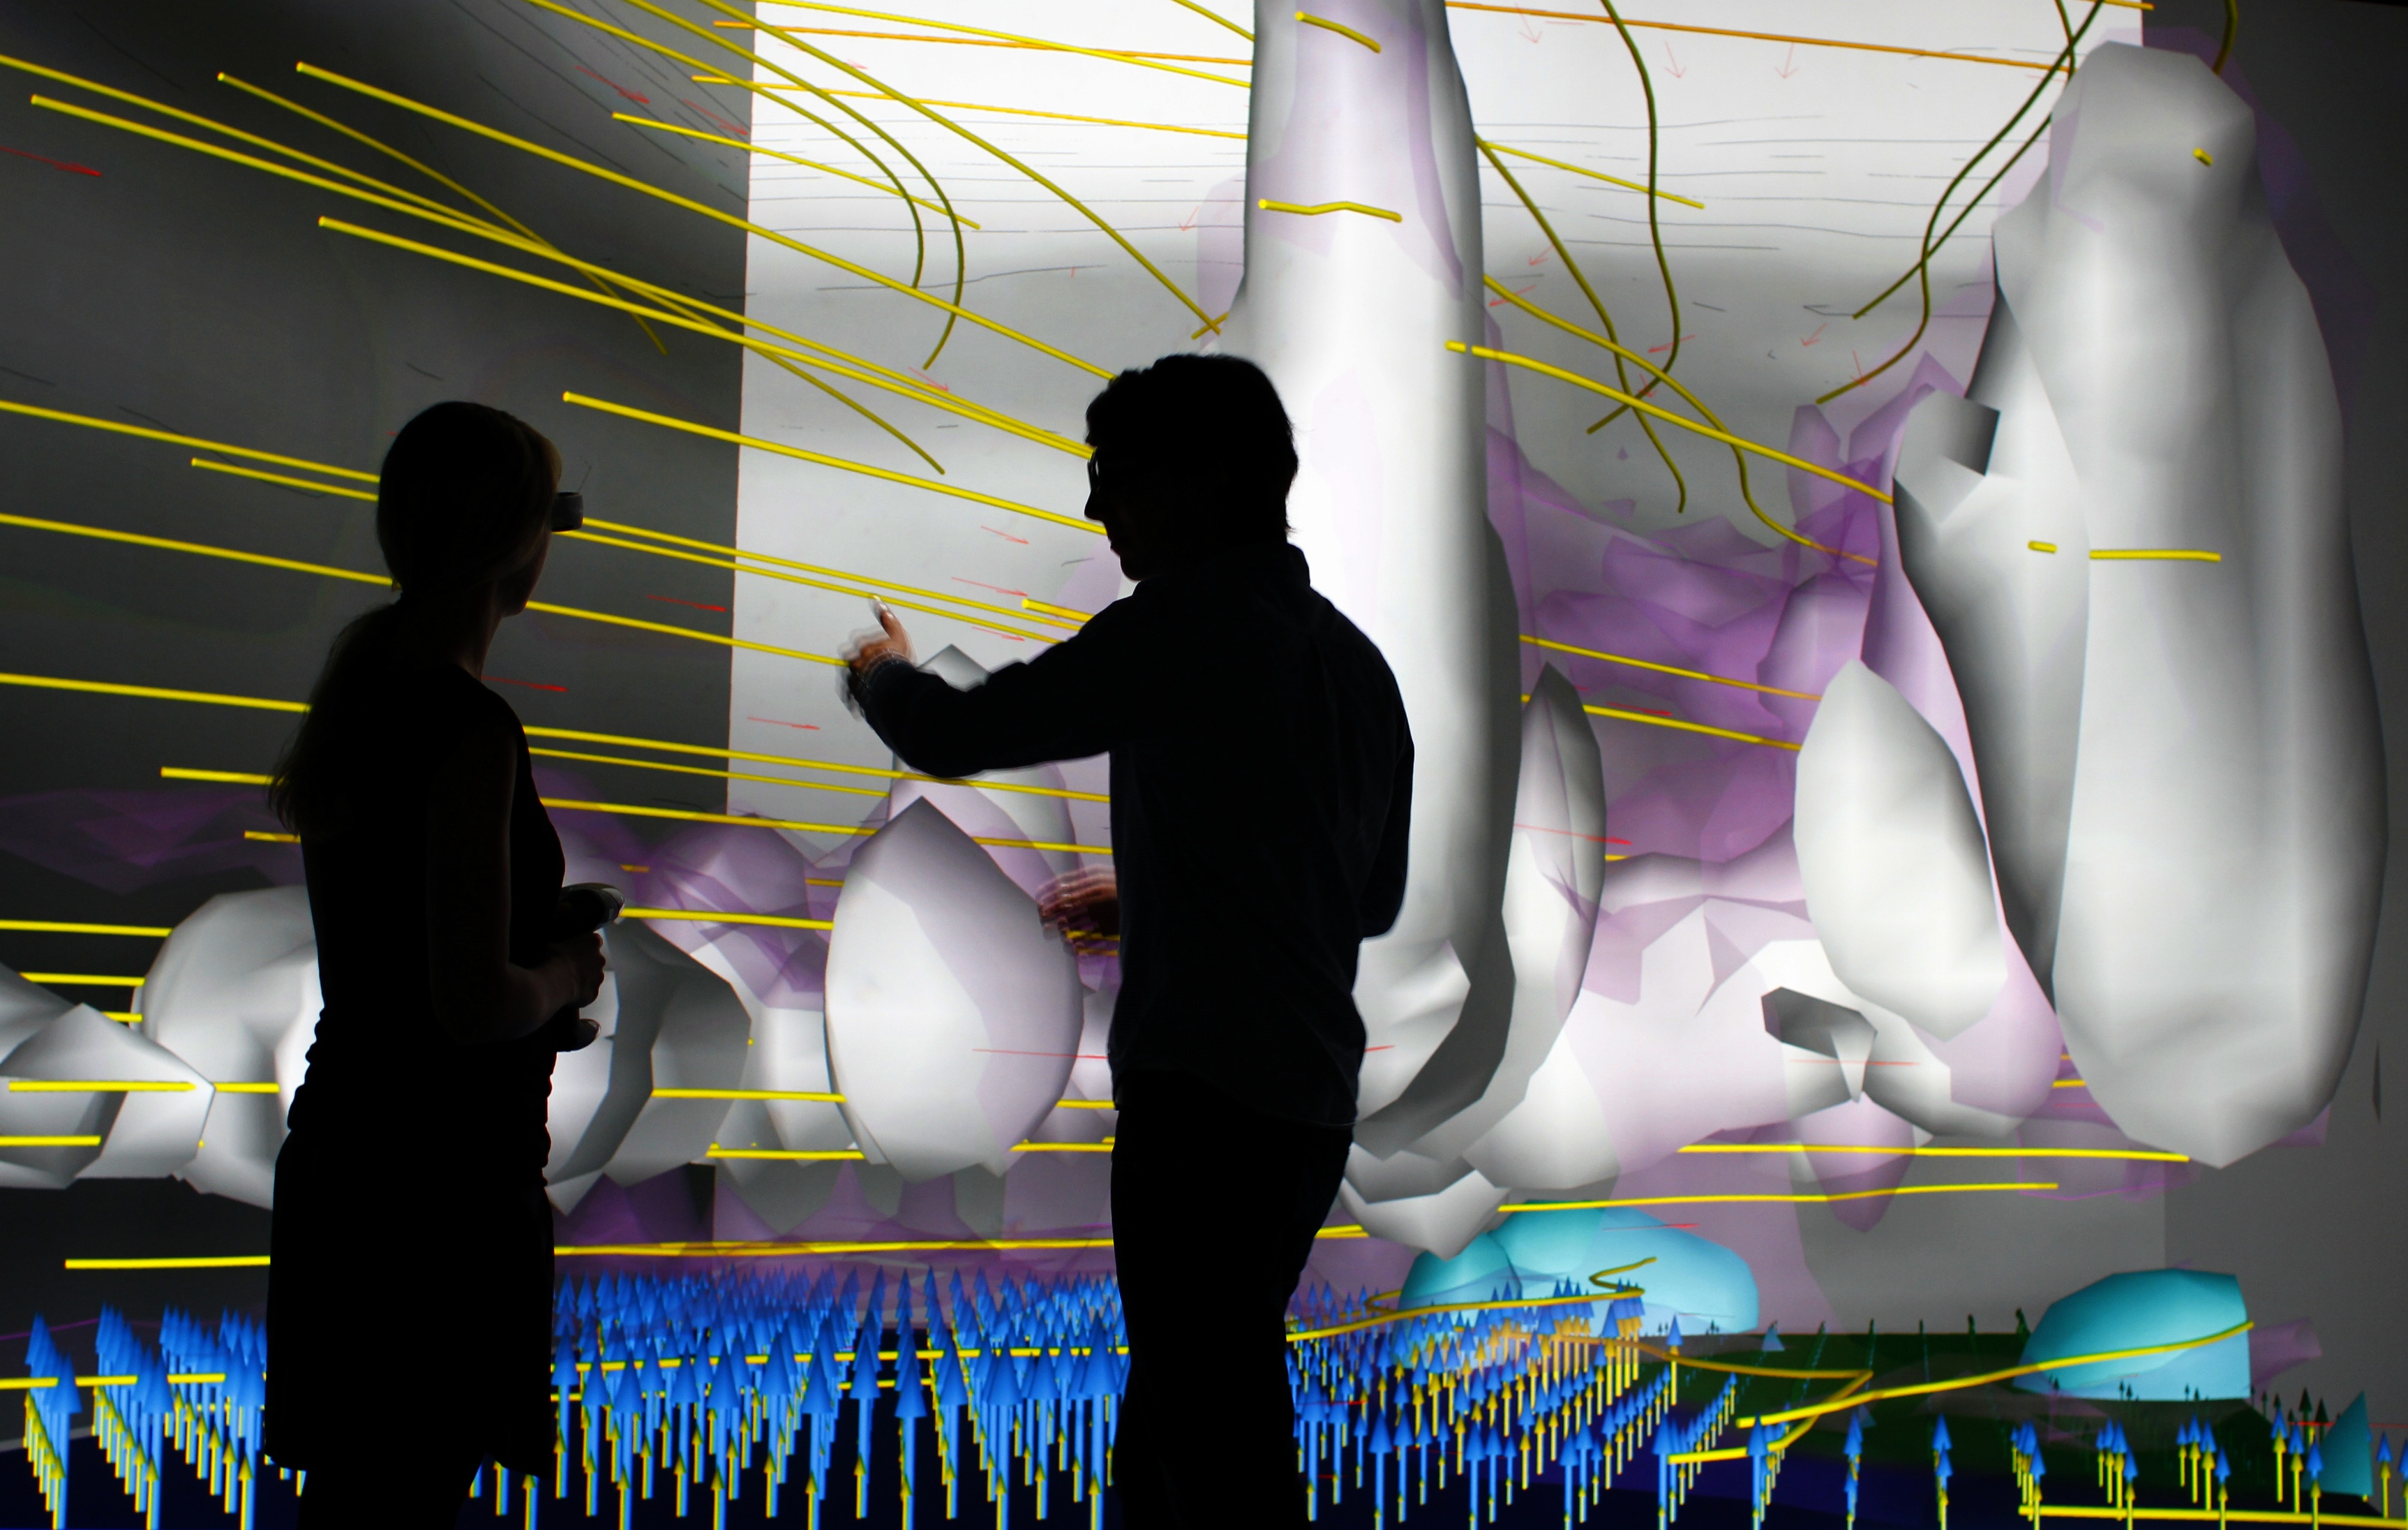
\includegraphics[width=\textwidth]{images/wind.png}
\caption{TODO Climate data}
\label{fig:wind}
\end{figure*}

\subsubsection{Pore-Scale}
\label{pore-scale}

Dmitry Naumov

\subsubsection{Nankou}
\label{nankou}

Feng Sun \cite{sun:ees}

\begin{figure}
  \includegraphics[width=\linewidth]{images/nankou.jpg}
\caption{TODO Nankou groundwater deteriation}
\label{fig:nankou}
\end{figure}

\subsubsection{Oman - Saltwater Intrusion}
\label{oman---saltwater-intrusion}

Marc Walther

\begin{figure}
  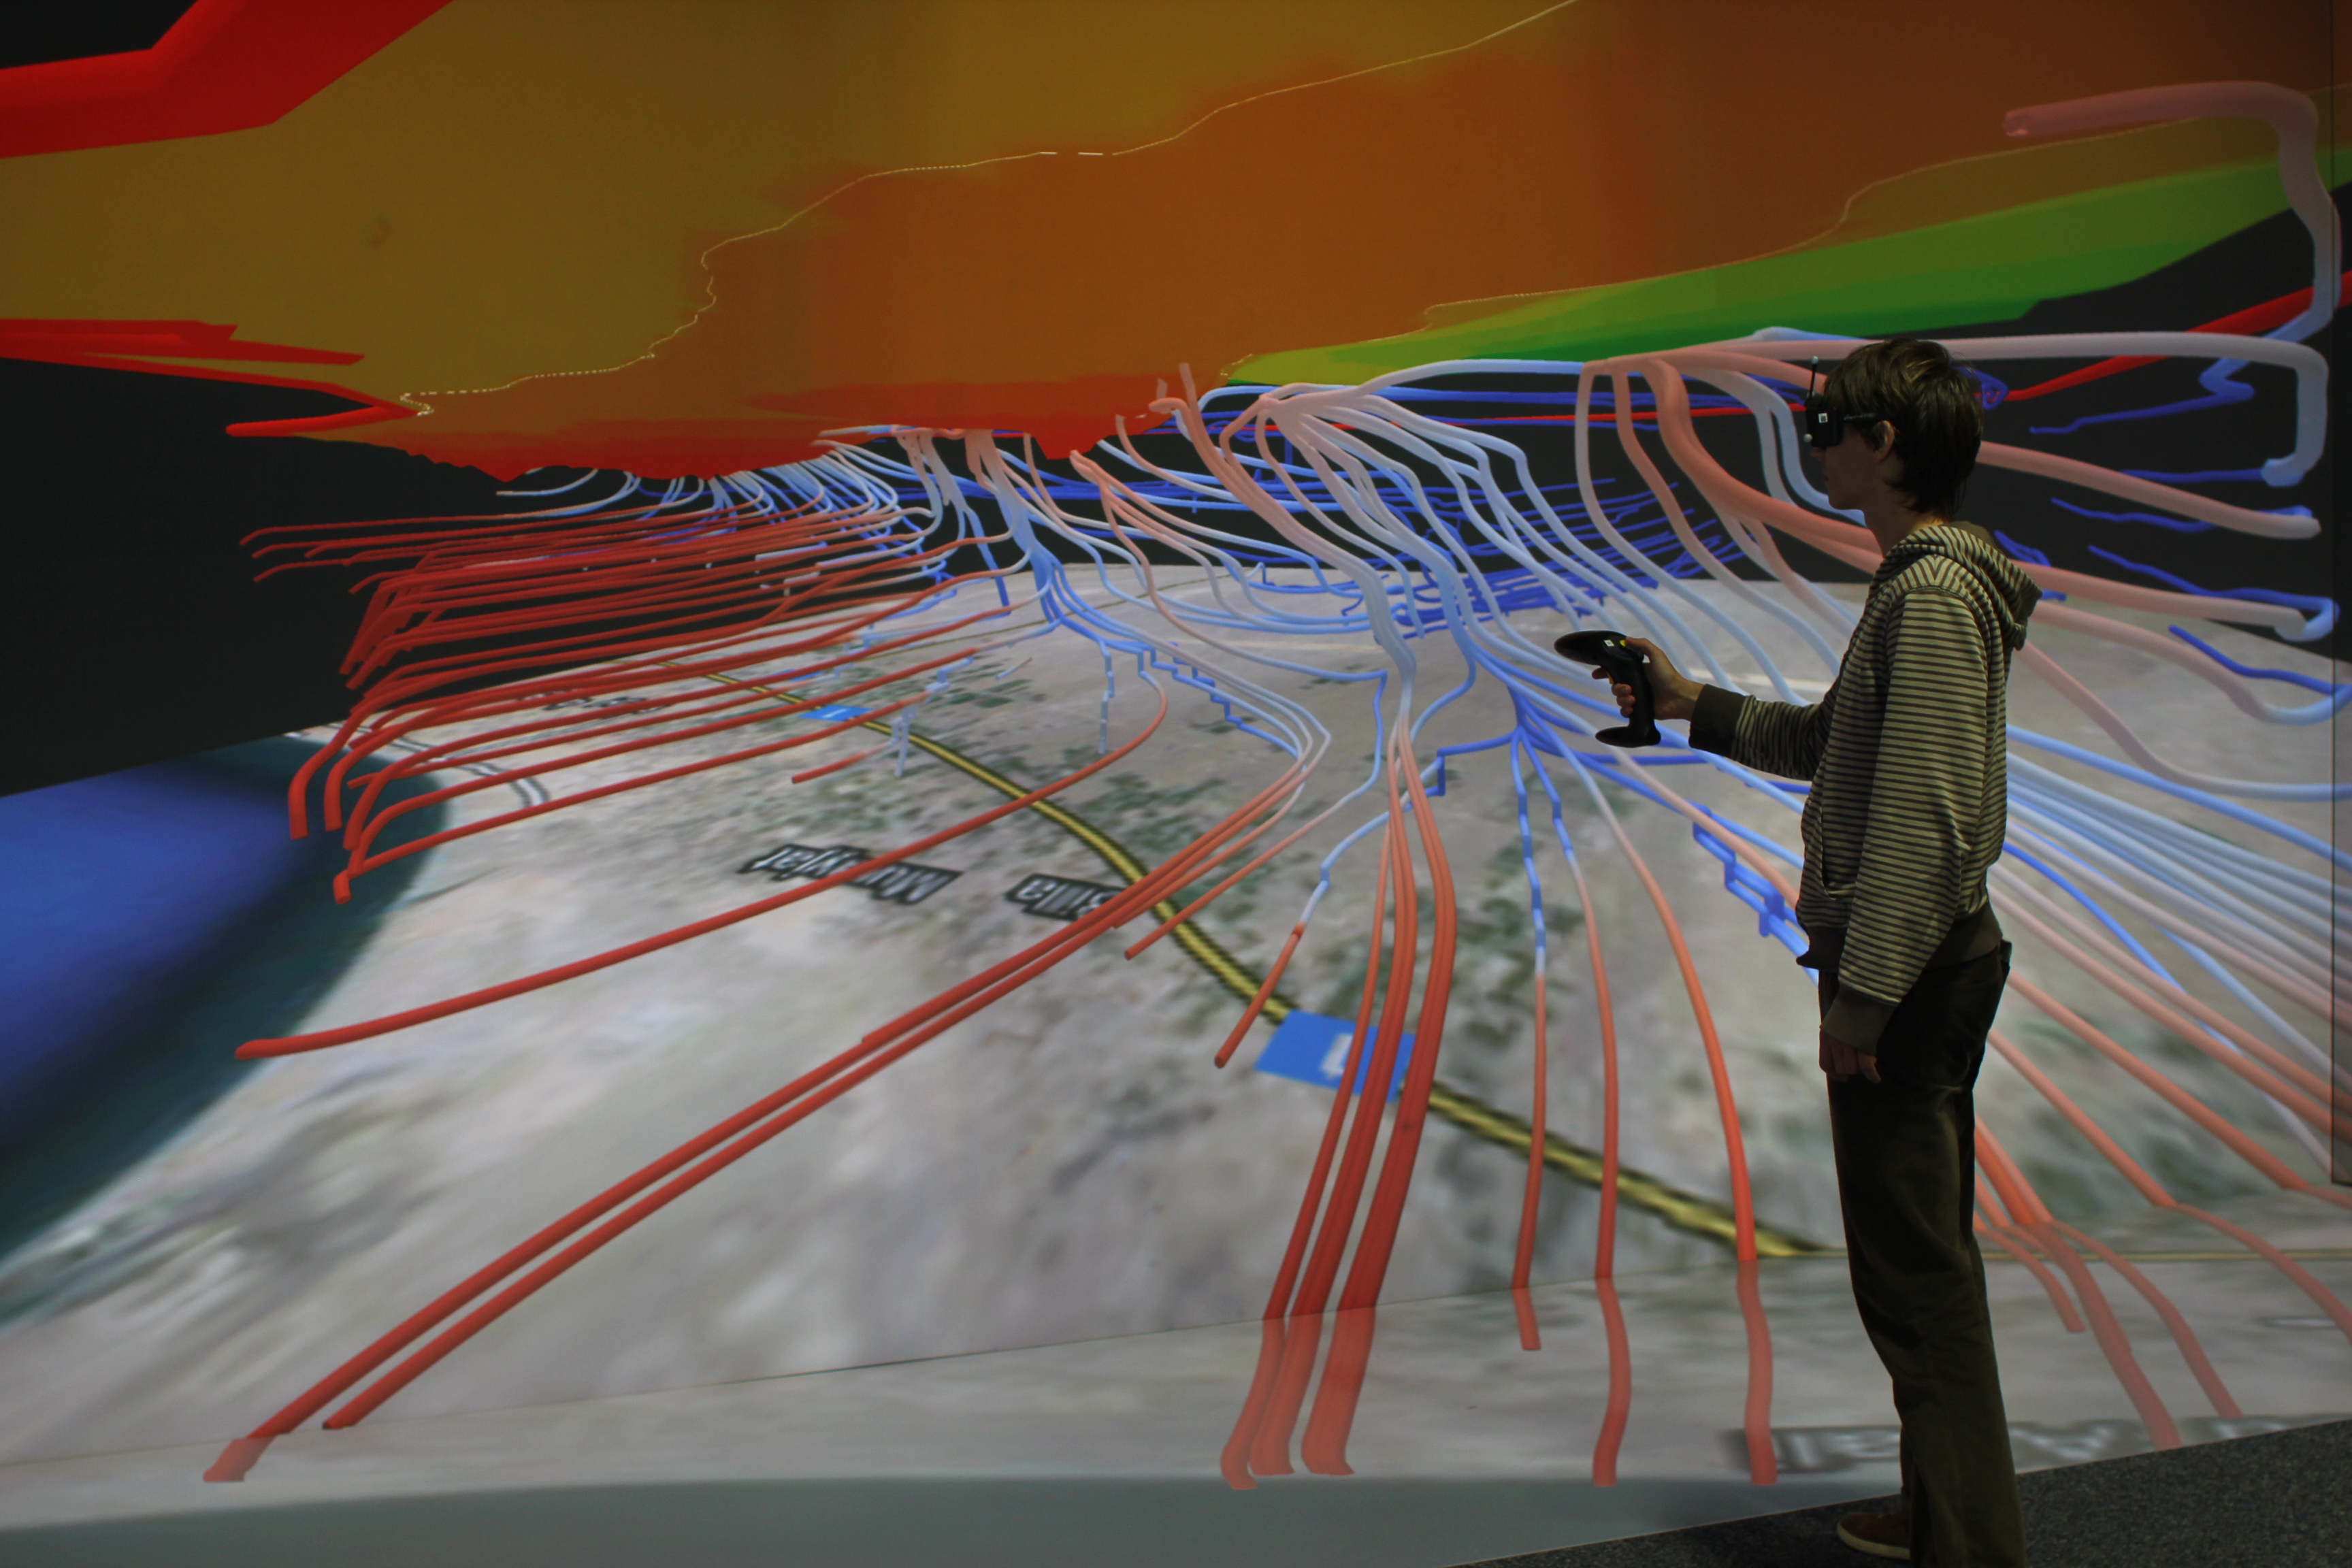
\includegraphics[width=\linewidth]{images/oman.jpg}
\caption{TODO}
\label{fig:oman}
\end{figure}

Using numerical models for the assessment of current and future states
of real world applications, aiding in the evaluation of various
management options, has become a standard - not only in environmental
sciences. Proper tools are needed to visualize the data properly for
analyzing and investigating measurements and modeling results. With
nowadays increasing density of available data and concurrently more and
more detailed model setups, this need has grown strongly. This trend is
also expressed through the ascending number of recent publications (
TODO TKs Saudi Arabien Model, \cite{sun:ees}, \cite{helbig:envirvis}) and the increasing scientific awareness
of this circumstance during conferences (eg. EnvirVis as part of
EuroVis). One of these case studies, a region scale study on density
driven flow in a coastal aquifer that is used as source for agriculture
irrigation, intensively made use of visualization options during model
setup, verification of the variable density process, and for the
transfer of knowledge to local authorities(\cite{walther:cam} \& \cite{walther:eesenvirvis}). Firstly, visualization was used to investigate plausibility of
the set up hydro-geological model, that was constructed based on an
extended inverse weighting distance interpolation\cite{walther:modelcare}. Secondly, large datasets of model calibration and long term
scenario simulations of the saltwater intrusion process were analyzed by
utilizing ParaView. ParaView was run on a parallel cluster computer to
omit bandwidth limitations to copy large data and to reduce
computational burden on standard desktop machines. Thirdly, results of
the modeling were visualized, which helped during discussions with
experts and tremendously aided in knowledge transfer during a visit of
Omani authorities from the Ministry of Regional Municipalities and Water
Resources. Additionally, throughout all states of model development,
calibration, scenario analysis, and result presentation, the VISLab was
utilized.

\subsubsection{TERENO-Bode}\label{tereno-bode}

Karsten Rink

\subsubsection{Saudi-Arabia - Groundwater
Flow}\label{saudi-arabia---groundwater-flow}

Thomas Kalbacher \cite{zehner:modelcare} and \cite{rink:modelcare}

\subsubsection{Streambed}\label{streambed}

Nico Trauth

\begin{figure}
  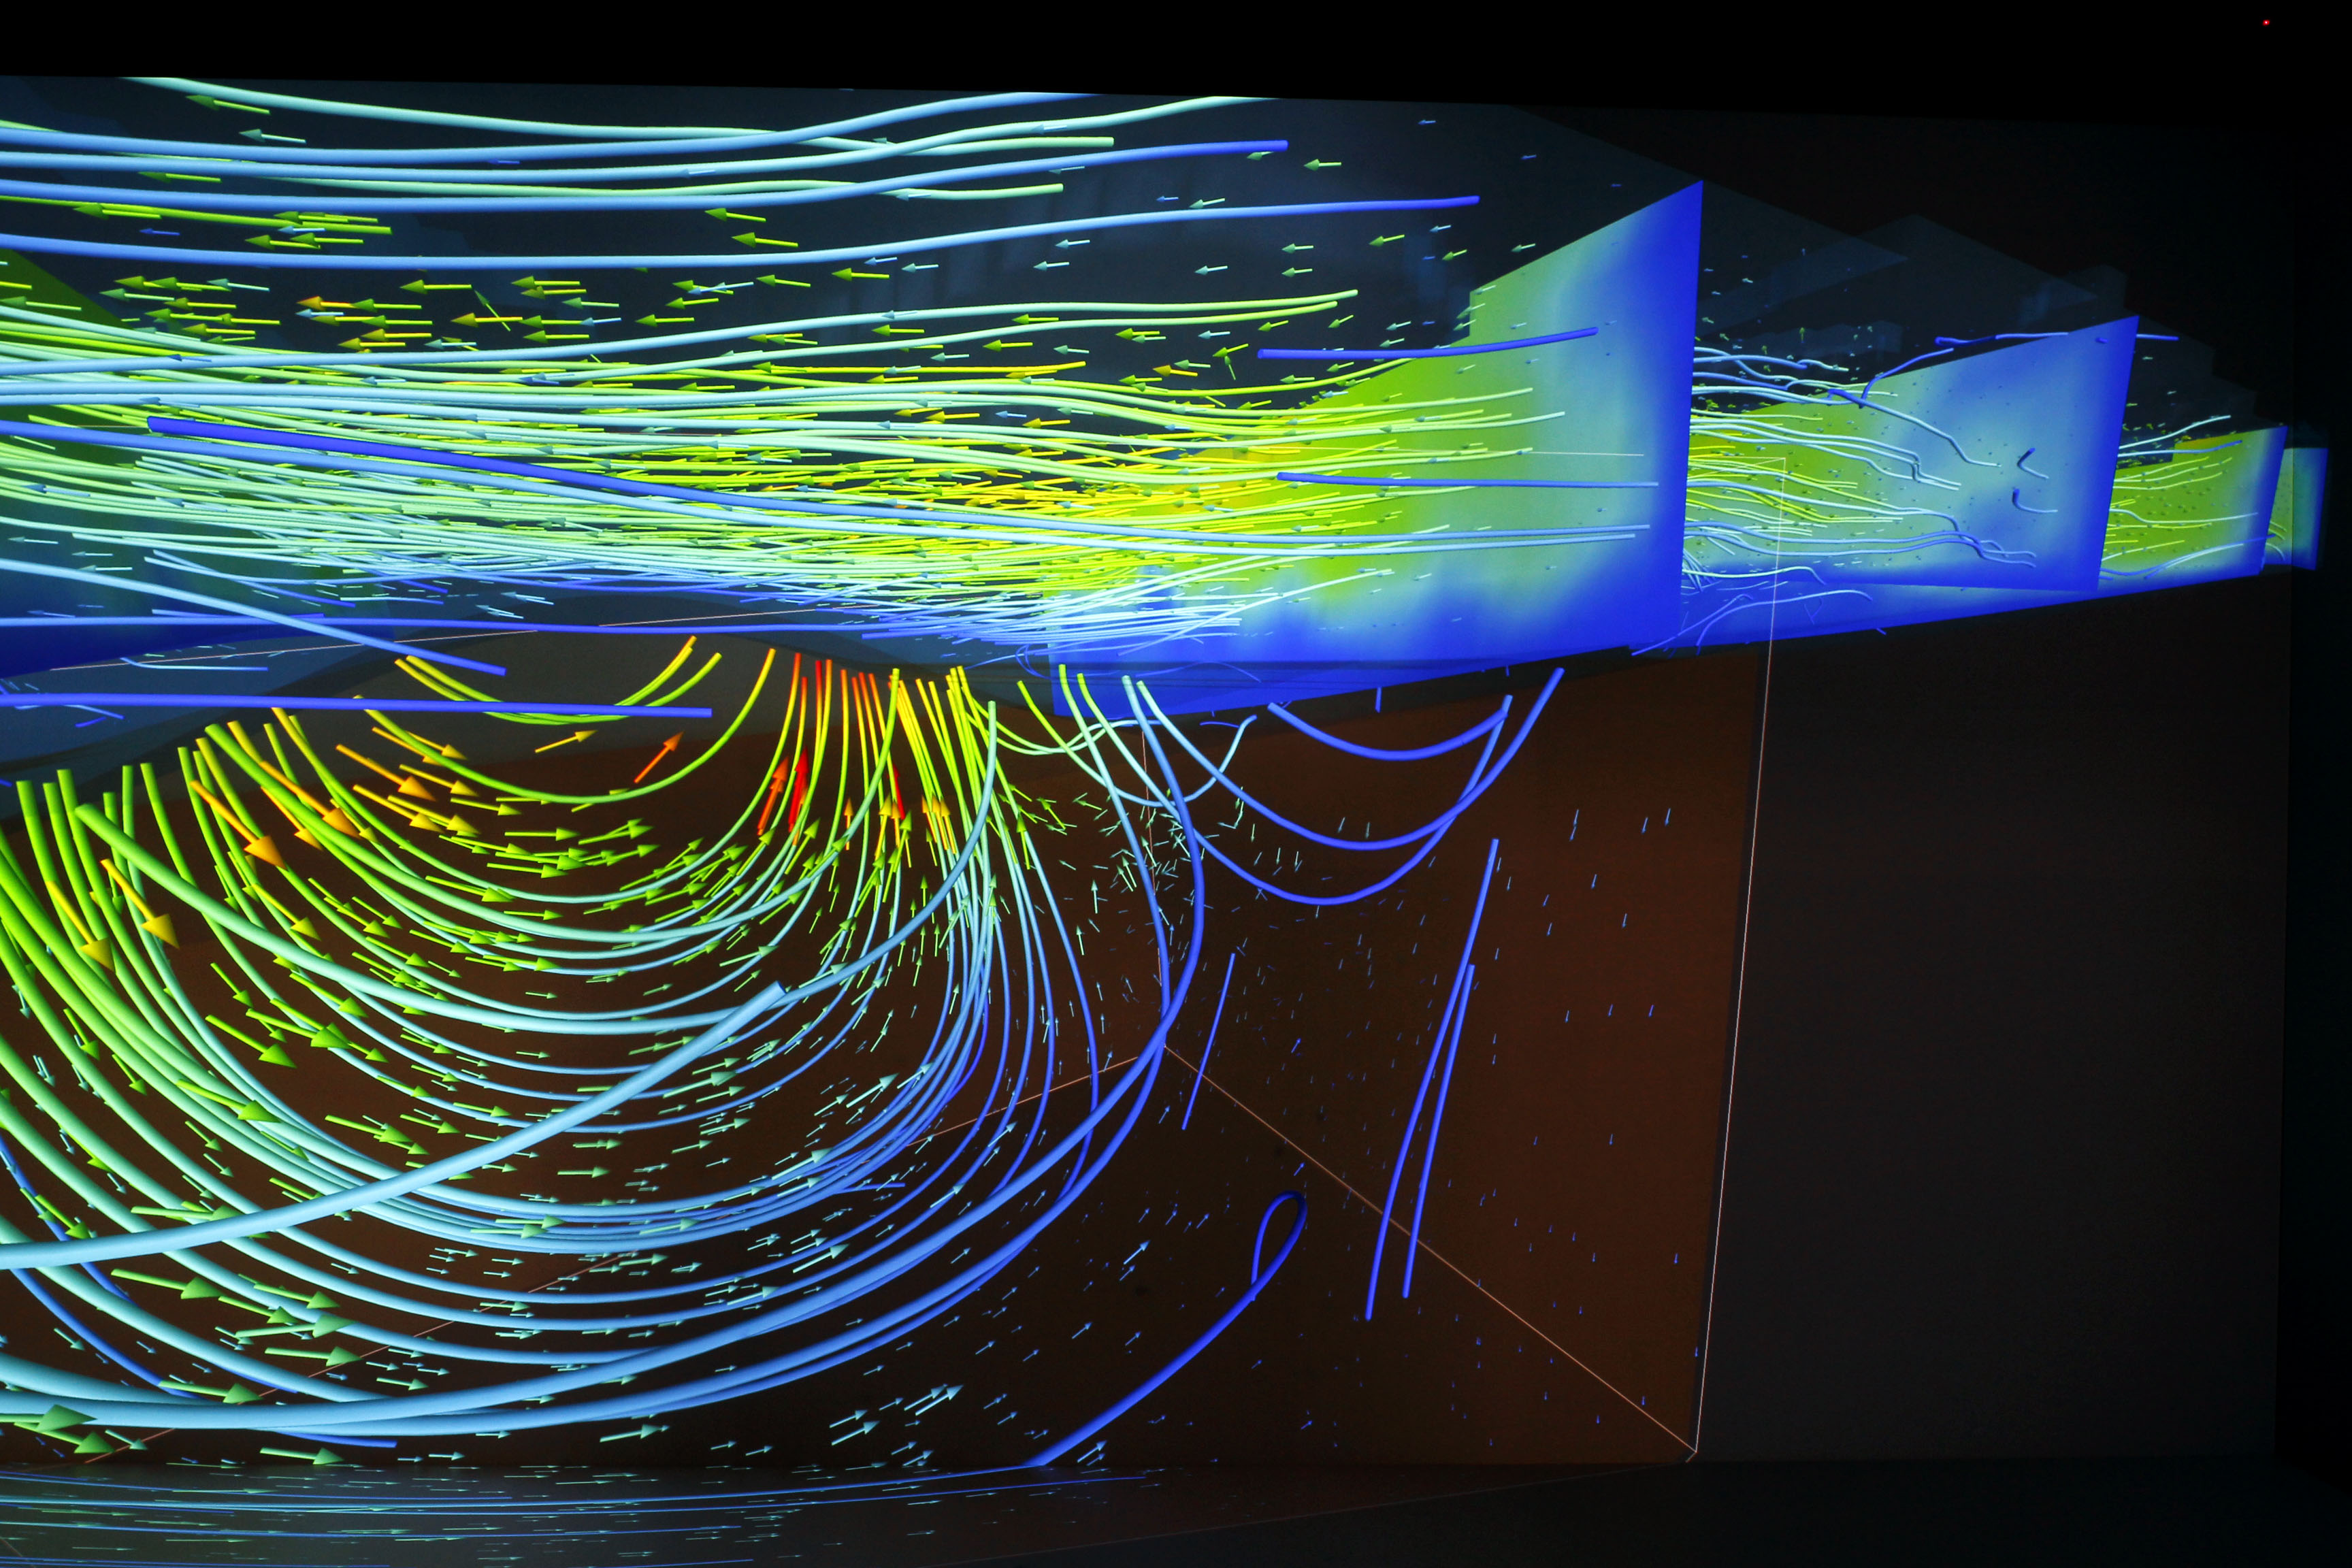
\includegraphics[width=\linewidth]{images/streambed.jpg}
\caption{TODO}
\label{fig:streambed}
\end{figure}

\subsection{Geosciences and Energy}\label{geosciences-and-energy}

In geosciences we have to deal with complex geological structures
containing different architectural elements such as layers, faults,
diapirs, fracture networks. Thermo-hydro-mechanical-chemical processes
under extreme thermodynamic conditions have to be considered for
utilizing geological reservoirs, e.g.~for geothermal energy (Zehner et
al. 2010).

\subsubsection{Gro{\ss}-Sch\"onebeck - Geothermal Energy}
\label{grouxdf-schuxf6nebeck---geothermal-energy}

Norihiro Watanabe

\subsubsection{Otway-Basin - CO2-Storage}
\label{otway-basin---co2-storage}

Jennifer Ziesch

\subsubsection{Thuringia Basin - Faults}
\label{thuringia-basin---faults}

Bj\"orn Zehner

\subsection{Landscape and Biodiversity}
\label{landscape-and-biodiversity}

Many man-made actions have an impact on landscapes as well as to
biodiversity surrounding us and this should be communicated to and
discussed with the public, so that people are aware of this fact.
Virtual Environments are very well suited for the integration and
visualization of various data within a unique geographic context for
discussion and decision making of different options (TODO Zehner 2010).

\subsubsection{Biodiversity in Rain Forests}
\label{biodiversity-in-rain-forests}

Andreas Huth Formind \cite{kohler:98}

\begin{figure}
  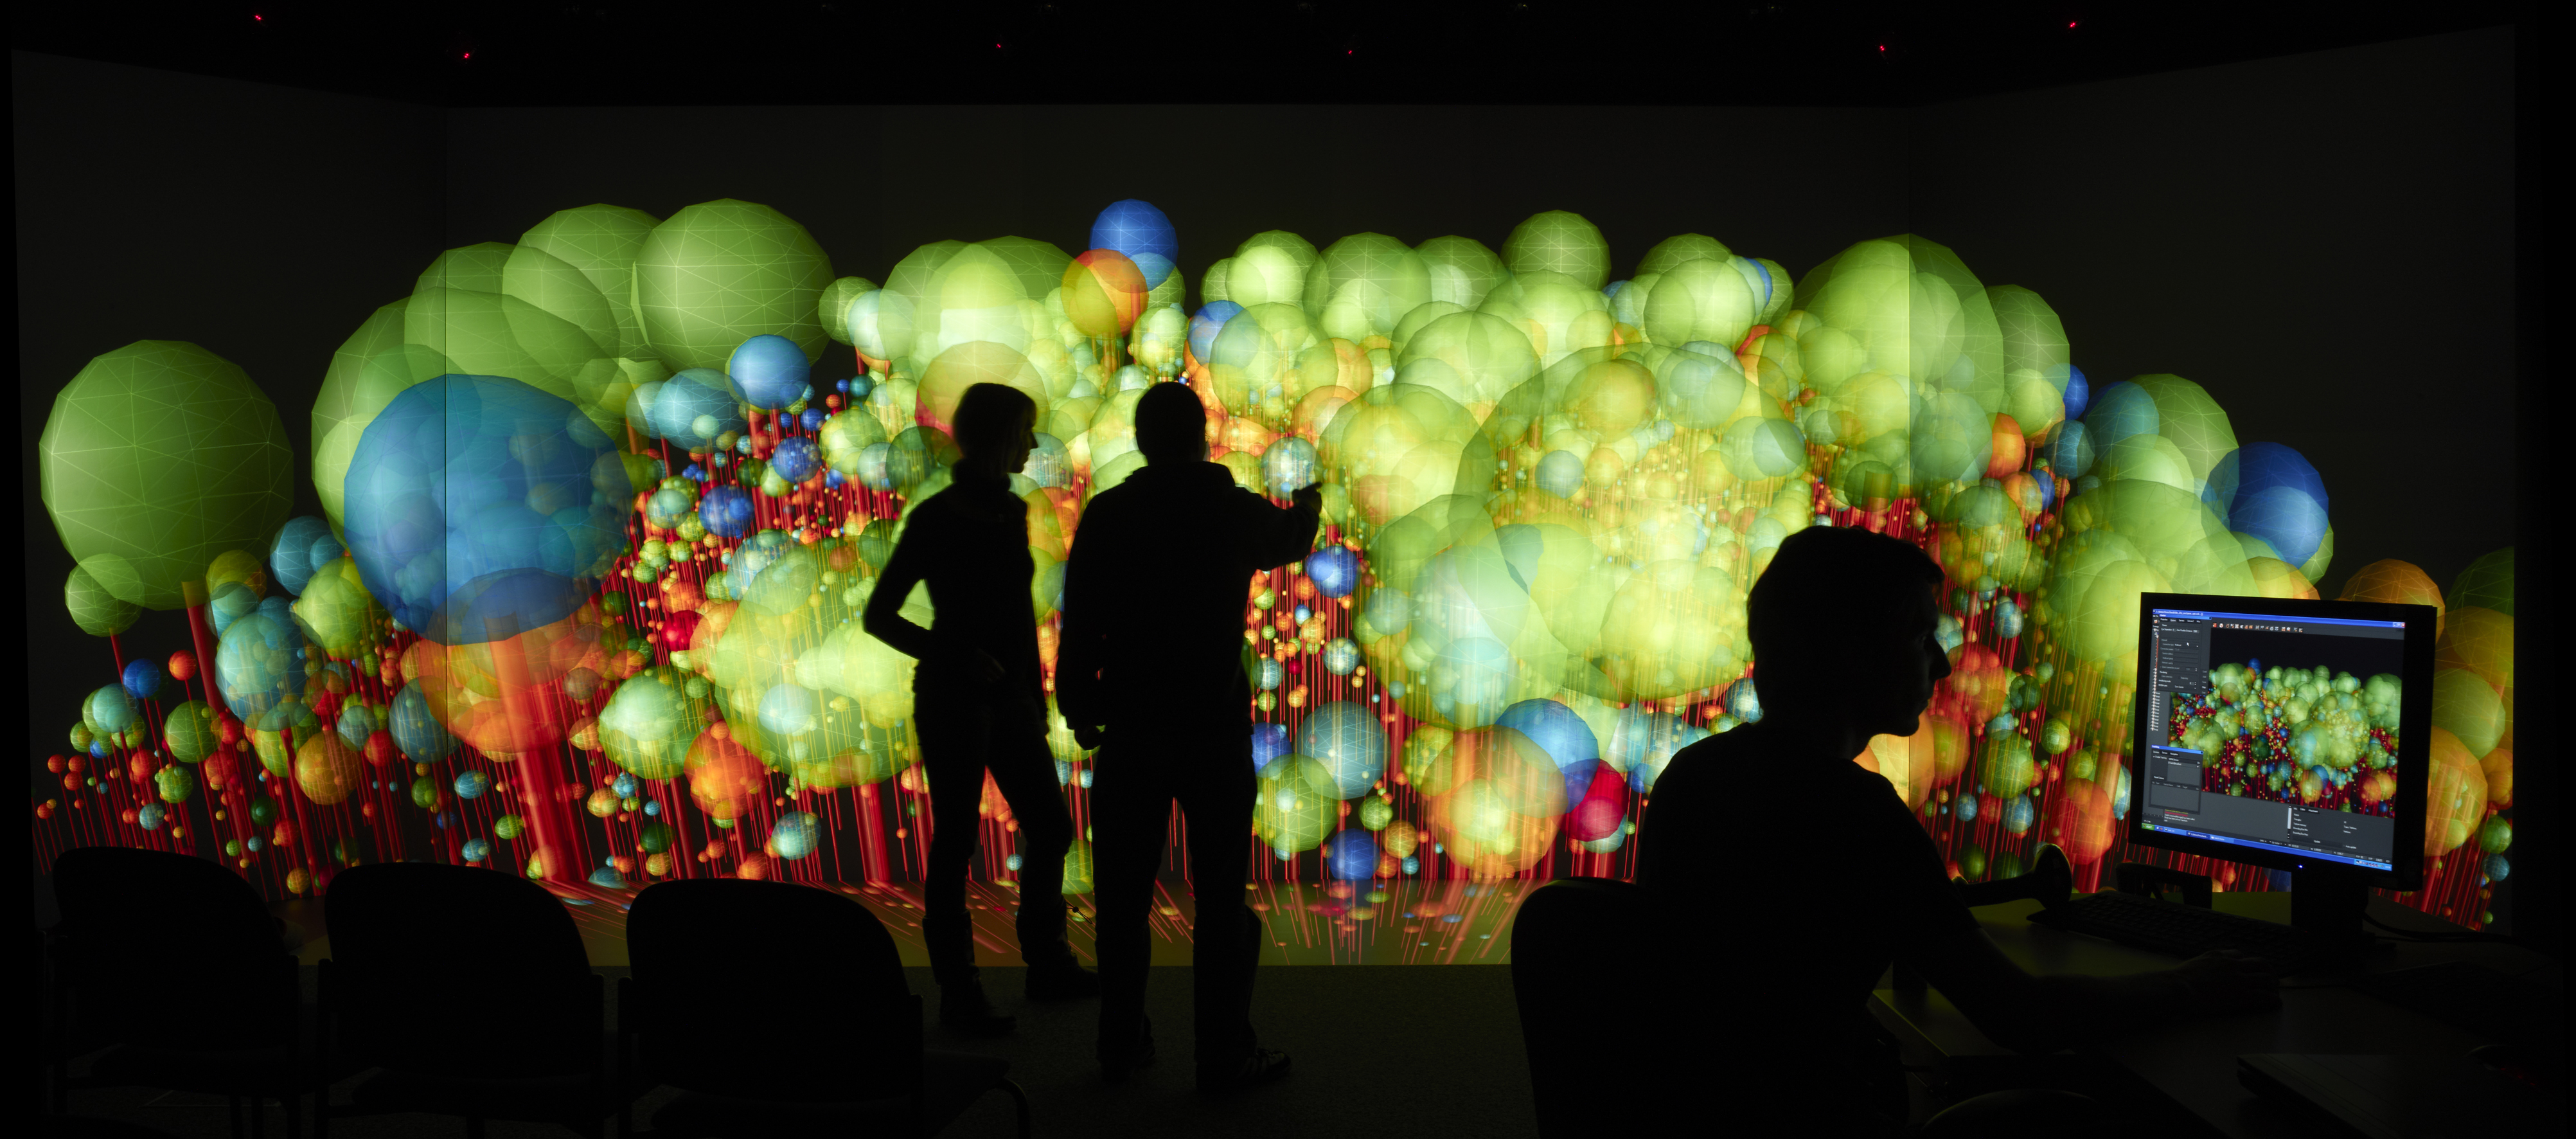
\includegraphics[width=\linewidth]{images/biodiversity.jpg}
\caption{TODO}
\label{fig:biodiversity}
\end{figure}

\subsubsection{Windpark Planning}
\label{windpark-planning}

Björn Zehner

\subsection{Urban Environments}
\label{urban-environments}

\subsubsection{Urban Vis}
\label{urban-vis}

Lars Bilke

\section{Future work}
\label{future-work}

For the future we want to integrate new visualization techniques to
better incorporate scientific visualization in the daily research work,
especially into high-performance computing (HPC). To achieve these goals
we will integrate visualization methods into simulation codes and simplify
the technical setup to unlock more fields of applications.

\subsection{In-situ visualization}
\label{in-situ-visualization}

In-situ or Co-visualization allows to create result analysis and
visualization as a part and during the simulation process. HPC systems
are getting more processing power, more memory and more
communication bandwidth every year. But not all of these capacities are
growing at an equal rate. Especially communication bandwidth can be the
limiting factor in various applications.

Normally the simulation process is tripartite: in the
\emph{preprocessing} the model of the simulation gets defined and all
input data gets prepared for the simulation run. Typically the
\emph{simulation} step produces large amounts of result data which are
then processed and analysed in the \emph{postprocessing} step. Usually
the postprocessing takes place on frontend-nodes of the HPC system or on
the users PC and storage capacity may be limited. In the latter case all
result data have to be transfered over the computer network. The analysed
data as the outcome of the postprocessing step is much smaller than the
simulation result data. Therefore the postprocessing should become
integrated into the simulation itself to avoid the communication bottleneck
and to transfer the analysed data only.

We will use the library Catalyst\footnote{Catalyst: \url{http://catalyst.paraview.org}} for
integration into OpenGeoSys. Catalyst is an extension of the
Visualization Toolkit (VTK) / ParaView. On the basis of a representative
example data set the user defines a visualization pipeline (either by a
script or interactively in ParaView) which is then executed after
defined time step intervals of the simulation. During simulation time
the user gets processed data as a result of the visualization pipeline,
images of the visualization and an interactive remote visualization in
ParaView.

Furthermore it should be possible to view the live visualization in the
VR environment of the TESSIN VISLab which is also connected to the EVE HPC
system of the UFZ.

By observing the simulation process it is possible to detect errors in
the input data early. The user can then cancel the simulation, adapt the
input data and restart the simulation. This conducts to savings in
compute and work time and to an effective iterative process of refining
and adapting the simulation. Because the in-situ visualization can be
run without user interaction it is also useful for software quality
management and benchmarking. Comparing visualization output and analyzed
data between different program versions can be very helpful to detect
errors in the code.

\subsection{Simplified hardware setup}
\label{simplified-hardware-setup}

Our current hardware setup limits the usable 3D applications to those
which can run in parallel and synchronized on a computer cluster. This
rules out the usage of commonly used software such as geographic
information systems (GIS). Novel high resolution projectors can help us
to reduce the number of projectors for our display from 13 to 8 in which
the main screen is driven by one 4K projector instead of six SXGA
projectors. This allows the usage of every 3D enabled application when
disclaiming the projection on the ground and side screens. The technical
implementation is currently under review.

%%%%%%%%%%%%%
%% ENDCONTENT
%%%%%%%%%%%%%

%
% For tables use
\begin{table}
% table caption is above the table
\caption{Please write your table caption here}
\label{tab:1}       % Give a unique label
% For LaTeX tables use
\begin{tabular}{lll}
\hline\noalign{\smallskip}
first & second & third  \\
\noalign{\smallskip}\hline\noalign{\smallskip}
number & number & number \\
number & number & number \\
\noalign{\smallskip}\hline
\end{tabular}
\end{table}


%\begin{acknowledgements}
%If you'd like to thank anyone, place your comments here
%and remove the percent signs.
%\end{acknowledgements}

% BibTeX users please use one of
%\bibliographystyle{spbasic}      % basic style, author-year citations
\bibliographystyle{spmpsci}       % mathematics and physical sciences
%\bibliographystyle{spphys}       % APS-like style for physics
\bibliography{vislab}   % name your BibTeX data base

\end{document}
% end of file template.tex

